%%%%%%%%%%%%%%%%%%%%%%%%%%%%%%%%%%%%%%%%% 
% University Assignment Title Page 
% LaTeX Template
% Version 1.0 (27/12/12)
%
% This template has been downloaded from:
% http://www.LaTeXTemplates.com
%
% Original author:
% WikiBooks (http://en.wikibooks.org/wiki/LaTeX/Title_Creation)
%
% License:
% CC BY-NC-SA 3.0 (http://creativecommons.org/licenses/by-nc-sa/3.0/)
% 
% Instructions for using this template:
% This title page is capable of being compiled as is. This is not useful for 
% including it in another document. To do this, you have two options: 
%
% 1) Copy/paste everything between \begin{document} and \end{document} 
% starting at \begin{titlepage} and paste this into another LaTeX file where you 
% want your title page.
% OR
% 2) Remove everything outside the \begin{titlepage} and \end{titlepage} and 
% move this file to the same directory as the LaTeX file you wish to add it to. 
% Then add \input{./title_page_1.tex} to your LaTeX file where you want your
% title page.
%
%%%%%%%%%%%%%%%%%%%%%%%%%%%%%%%%%%%%%%%%%
%\title{Title page with logo}
%----------------------------------------------------------------------------------------
%	PACKAGES AND OTHER DOCUMENT CONFIGURATIONS
%----------------------------------------------------------------------------------------

\documentclass[12pt]{article}
\usepackage[english]{babel}
\usepackage[utf8x]{inputenc}
\usepackage{amsmath}
\usepackage{graphicx}
\usepackage{subcaption}
\usepackage{hyperref}
\usepackage{enumitem}
\usepackage{minted}
\usepackage{cite}
\usepackage{multirow}
\usepackage[colorinlistoftodos]{todonotes}

\begin{document}

\begin{titlepage}

\newcommand{\HRule}{\rule{\linewidth}{0.5mm}} % Defines a new command for the horizontal lines, change thickness here

\center % Center everything on the page
 
%----------------------------------------------------------------------------------------
%	HEADING SECTIONS
%----------------------------------------------------------------------------------------

\textsc{\LARGE Università degli studi di Milano-Bicocca}\\[1cm] % Name of your university/college
\textsc{\Large Advanced Machine Learning }\\[0.3cm] % Major heading such as course name
\textsc{\large Final Project}\\[0.1cm] % Minor heading such as course title

%----------------------------------------------------------------------------------------
%	TITLE SECTION
%----------------------------------------------------------------------------------------

\HRule \\[0.4cm]
{ \huge \bfseries Electical Motor Temperature}\\[0.2cm] % Title of your document
\HRule \\[1.5cm]
 
%----------------------------------------------------------------------------------------
%	AUTHOR SECTION
%----------------------------------------------------------------------------------------

\large
\emph{Authors:}\\
Federico Moiraghi - 799735 - f.moiraghimotta@campus.unimib.it \\
Pranav Kasela     - 846965 - p.kasela@campus.unimib.it \\
Roberto Berlucchi - 847939 - r.berlucchi@campus.unimib.it \\
[0.5cm] % Your name

% If you don't want a supervisor, uncomment the two lines below and remove the section above
%\Large \emph{Author:}\\
%John \textsc{Smith}\\[3cm] % Your name

%----------------------------------------------------------------------------------------
%	DATE SECTION
%----------------------------------------------------------------------------------------

{\large 2019 - 2020}\\[1cm] % Date, change the \today to a set date if you want to be precise

%----------------------------------------------------------------------------------------
%	LOGO SECTION
%----------------------------------------------------------------------------------------


\includegraphics{imgs/logo.png}\\[1cm] % Include a department/university logo - this will require the graphicx package
 
%----------------------------------------------------------------------------------------

\vfill % Fill the rest of the page with whitespace

\end{titlepage}


\begin{abstract}
  The present Report is a summary of methodologies used to predict the temperature of various part of a prototype electrical motor after some tests on a bench. The resulting model have to yield acceptable predictions and to be light enough to be used by the car itself during its daily use: autos can start cooling components before the temperature grows critically (first task) or can estimate temperature without a specific sensor (second task), due to its cost and weakness, knowing only basic environmental information.
\end{abstract}

\section{Introduction}
The data set comprises several sensor data collected from a permanent magnet synchronous motor (PMSM) deployed on a test bench. The PMSM represents a German OEM's prototype model and test bench measurements were collected by the LEA department at Paderborn University.

Recordings are sampled at a frequency of $2Hz$ and are divided in various profiles, with a total of $998070$ observations. Each profile indicates a different test session, that last from one to six hours.

Input variables are:
\begin{itemize}[topsep=0ex, noitemsep]
    \item \textbf{Ambient temperature}: as measured by a thermal sensor located close to the stator;
    \item \textbf{Coolant temperature}: the motor is water cooled and the measurement is taken at outflow;
    \item The current and voltage are transformed through a $dq0$ transformation in a d-q coordinate system, it basically converts a three phase balanced reference system (in an AC system) into 2 coordinates, denoted by d and q, via a rotating reference frame with angle $\theta$.
    The currents are denoted by \textbf{i\_d} and \textbf{i\_q} and the voltages are denoted by \textbf{u\_d} and \textbf{u\_q};
    \item \textbf{Motor speed}.
\end{itemize}

Target variables are:
\begin{itemize}[topsep=0ex, noitemsep]
    \item \textbf{pm}: Permanent Magnet surface temperature, representing the rotor temperature (measured with an infrared thermography unit).
    \item \textbf{stator\_yoke}, \textbf{stator\_tooth}, \textbf{stator\_winding}: temperatures of the corresponding components measured with a thermal sensor.
\end{itemize}
In some of the variables, Gaussian noise is introduced to simulate real world driving cycles. Being sensors data, missing values are replaced by the provider with the previous one, causing some flat areas when sensors fall offline for a long period. 

The main objective is to create a lightweight model to predict the \verb|pm| and \verb|stator|s variables, minimizing the MSE (because the model needs to be deployed with best cost-precision ratio); a secondary goal is to predict more accurately higher temperature than the lower temperature using a modified loss.

\section{Datasets}
The data set can be found on Kaggle\footnote{\href{https://www.kaggle.com/wkirgsn/electric-motor-temperature}{https://www.kaggle.com/wkirgsn/electric-motor-temperature}}. From the data set the \verb|torque| feature is immediately excluded, as it is deemed unreliable from the data set provider itself.
\begin{figure}[!h]
    \centering
    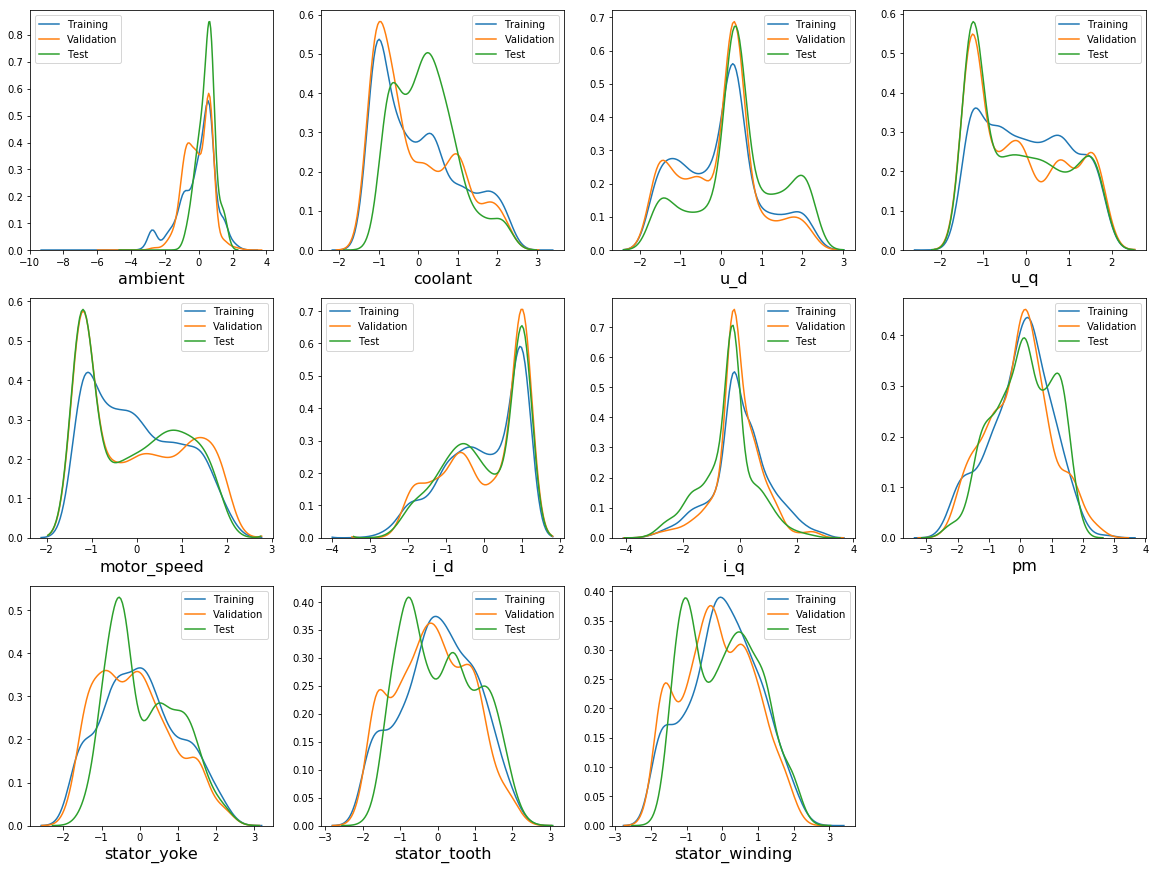
\includegraphics[width=\linewidth, height=10cm]{imgs/dist_plot.png}
    \caption{Distribution of the variables grouped by the division}
    \label{fig:dist_plot}
\end{figure}\\
The data set is divided into train, validation and test set: validation data consists of \verb|profile_id|s $20, 31, 46, 54, 62, 70, 79, 72$; the test set profiles are $35$ and $42$ and the training set consists of all the other profiles. Their relative distributions are plotted in the Figure \ref{fig:dist_plot}.

Figure \ref{fig:corrplot} shows the correlation between the variables and it is seen that the target variables are highly correlated among themselves, in particular the \verb|stator|s variables.
\begin{figure}[!h]
    \centering
    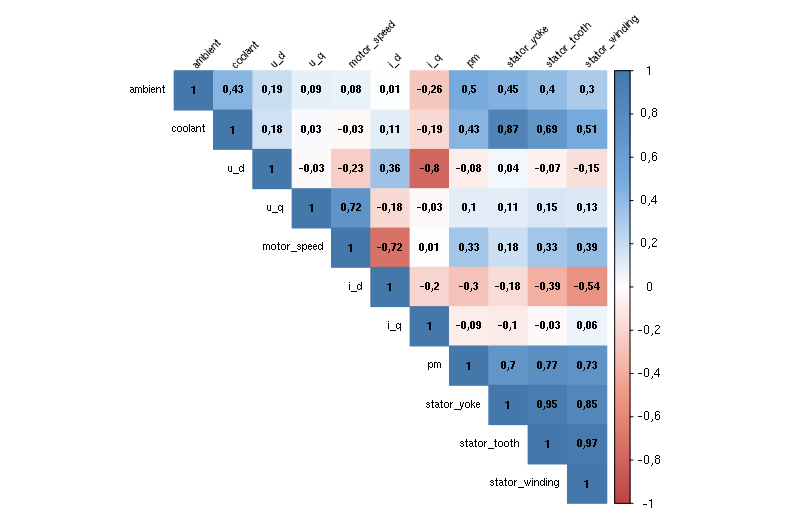
\includegraphics[width=\linewidth, height=7cm]{imgs/corrplot.png}
    \caption{Correlation Plot of the considered variables}
    \label{fig:corrplot}
\end{figure}

Data was already standardized by the provider (to anonymize data), but variables do not have a normal distribution, thus a further normalization between 0 and 1 (only on the training set) is applied.\\
% @Momo: questo lo diciamo dopo (dataloaders), personalmente lo toglierei 
% For each profile the data set is modified: to each row the lagged features are concatenated, the number of lags to keep can be changed, after this procedure the rows of all the profiles are united and shuffled through a custom data loader.

\section{The Methodological Approach}
Different \textit{Deep Learning} architectures are tried in order to compare them and choose the most suitable model to the problem: each model is built using \mintinline{python}|pytorch| and optimized with an Auto-ML algorithm using \mintinline{python}|sherpa| optimization library. In particular the \textit{Gaussian Process} (GP) surrogate model is used with the \textit{Expected Improvement} (EI) acquisition function to have a better exploration during the optimization.

Each model is optimized using Adam optimizer, using standard \textit{Mean Squared Error} (MSE) as loss function in a first trial, and then re-optimized using a custom weighted-version that assigns a triple importance to temperatures that surpass the value of the median (computed on the train set).
%??? aah sì, io avevo messo a caso 0.5 che è il valore medio del range ahahahaha

\subsection{Dataloaders}
To avoid giving all input and output matrix to the model  % (which has a side-effect: it fills both RAM and GPU memory and crashes everything)
, two ad-hoc dataloaders are programmed to optimize the learning process.
Belonging to various independent series, data is represented internally as a sequence of tuples $<\text{id}_{serie}, \text{id}_{observation}>$ so that can be easily shuffled and yielded to the model (without side-effects) using an arbitrary-large batch size.

\paragraph{First Task}
To accomplish the first task, data is given to the algorithm so that input matrix contains all values of all features and target variables throughout the temporal window (starting from an arbitrary moment in the past $t_{-max}$ (the maximum lag) to the previous observation $t_{-1}$), while target vector contains following values of only target variables at time $t_0$.

\paragraph{Second Task}
For the second task instead, dataloaders yield a input matrix containing only features values for a window time starting in a moment $t_{-max}$ to $t_0$; in addition a vector of values of target variables at time $t_0$ is given as ground truth: it's a real time prediction of the target and in this case there is a unique model which predicts all four targets.

\subsection{Models}
All models are implemented as Sequence to Value (Seq2Val) so that the training process can be paralleled and shuffled, with improvements in both speed and quality.
In addition, a Sequence to Value model can be easily rewritten as Sequence to Sequence (Seq2Seq), providing real-time information to the driver.

\paragraph{RNN}
In order to accomplish both tasks with a lightweight model easily usable by a car, a simple Recurrent Neural Network is implemented: this model is provided with one hidden layer that depends on both current data and previous observations, and uses it to estimate the target variables.
After the hidden layer, data flows through two independent feed-forward neural networks (with two layers both) to estimate values for \verb|pm| and \verb|stator|s variables: this approach is justified by the higher correlation between \verb|stator| temperatures and lower correlation with \verb|pm|.

Which layer (the previous input, the estimated output or the embedding) the RNN yields to the next step and how to use this information (where it is linked) are parameters settable in the model construction and optimized through Auto-ML; in addition, \textit{learning rate}, number of neurons per hidden layer, and length of the input sequence are optimized in the same way: to do so, the \mintinline{python}|Custom_RNN.forward()| method is implemented recursively to make it as adaptable as possible.

\paragraph{LSTM and GRU}
Two more type of recursive neural architecture are tested, the first one uses a LSTM layer while the other uses a GRU layer instead.
For the first task two independent models are created: one to predict only the \verb|pm| variable and one to predict the 3 \verb|stator| variables; time window size is fixed to 60 lags: it does not need to be optimized since the LSTM and GRU should automatically ``understand'' how many lags are important.

The model is pretty simple (as required by the task): it has one recurrent layer (either LSTM or GRU) followed by two fully connected layers, of which the second one can be omitted if the number of neurons is 0; lastly there is the output layer which has one neuron while predicting \verb|pm| and three neurons while predicting \verb|stator|.
During the second task all the four targets are predicted together.

The hyperparameter optimizer needs to optimize the number of hidden units, the number of neurons for each fully connected layer, the learning rate and the batch size of the data.
The objective score is the MSE and it is calculated, after one epoch of training, on the validation set.

\paragraph{CNN}
%roby explain your convolution idea! of course i do. fell free to add or modify :)
A CNN model is also tested, even though the number of parameters increases compared to the other approach described before.

For the first task, the model has 2 Convolutional layers, each one followed by a Max Pooling layer; the last convolution-pooling block is flattenized and followed by 2 Fully Connected layer and then the output layer. The second Convolutional and Fully Connected layers can be omitted if the number of filters or neurons are 0. For the second task the architecture is simplified: poolings are removed.
 
The convolution happens on the vectors that contain all the variables for each specific time in % $[t_{current-lag}, t_{current-1}]$, where $t_{current}$ is the time at which the target needs to be predicted and lag is the temporal window that the model can see.
$[t_{-max}, t_{-1}]$.
Basically this model is a lighter version of a FC model (it has less number of weights) and it extracts the most relevant features to pass to the FC layers.
The temporal window is the same used by the LSTM model.

In this architecture the hyperparameters to optimize are the stride and kernel of the convolutions, the number of neurons for each FC layer, the learning rate and the batch size.

% This is the central and most important section of the report. Its objective must be to show, with linearity and clarity, the steps that have led to the definition of a decision model. The description of the working hypotheses, confirmed or denied, can be found in this section together with the description of the subsequent refining processes of the models. Comparisons between different models (e.g. heuristics vs. optimal models) in terms of quality of solutions, their explainability and execution times are welcome. 
\section{Results and Evaluation}
 
\subsection{First Task}
In the Figure \ref{fig:automl_mse} results of hyper-parameter optimization are shown: for both models one predicting the \verb|pm| variable and the other predicting the three \verb|stator| variables. RNN is excluded because of it's poor performance (loss is two order of magnitude bigger) when compared to the other three models.

Results of the model on Training, Validation and Test are reported on the Table \ref{tab:first}, in this case all the output variables are concatenated together and a general loss is calculated.
\begin{table}[!h]
  \centering
  \begin{tabular}{|l|c|c|c|c|c|c|}
    \hline
           & \multicolumn{3}{|c|}{MSE}      & \multicolumn{3}{|c|}{Weighted MSE} \\
    \hline
    Models & Train   & Validation & Test    & Train   & Validation & Test \\
    \hline
    RNN    & 1.82e-3 & 2.17e-3    & 4.46e-3 & 4.21e-3 & 4.18e-3    & 2.55e-3\\
    CNN    & 2.32e-5 & 2.28e-5    & 2.39e-5 & 1.78e-5 & 1.80e-5    & 1.98e-5\\
    GRU    & 1.29e-5 & 1.24e-5    & 1.28e-5 & 2.42e-5 & 2.18e-5    & 2.48e-5\\
    LSTM   & 0.98e-5 & 0.96e-5    & 1.00e-5 & 2.20e-5 & 2.00e-5    & 2.23e-5\\
    \hline
  \end{tabular}
  \caption{Results on Training, Validation and Test Set for the first task. Values can change (in a small range) due to stochasticity of algorithms.}
  \label{tab:first}
\end{table}
\begin{figure}[!h]
    \centering
    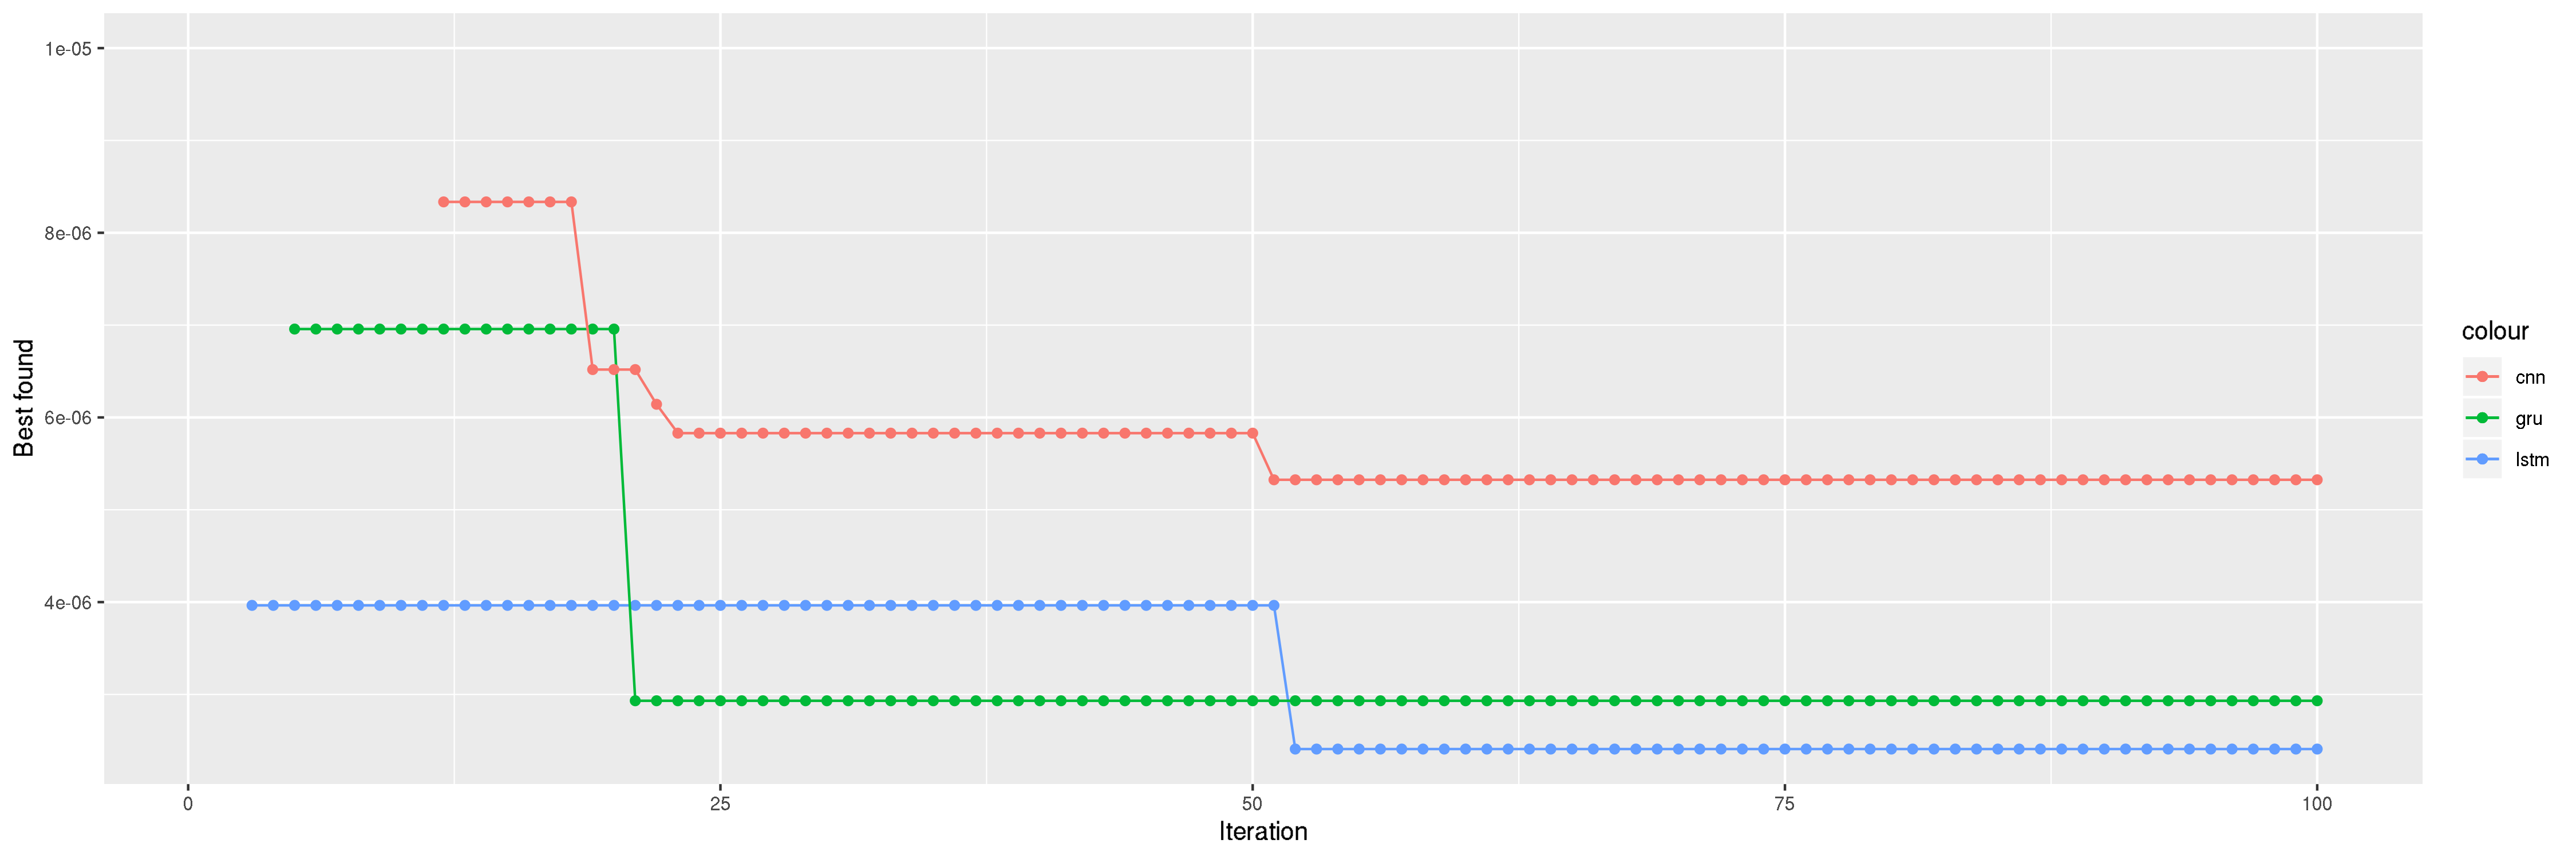
\includegraphics[width=\linewidth, height=4cm]{imgs/comparison_MSE.png}
    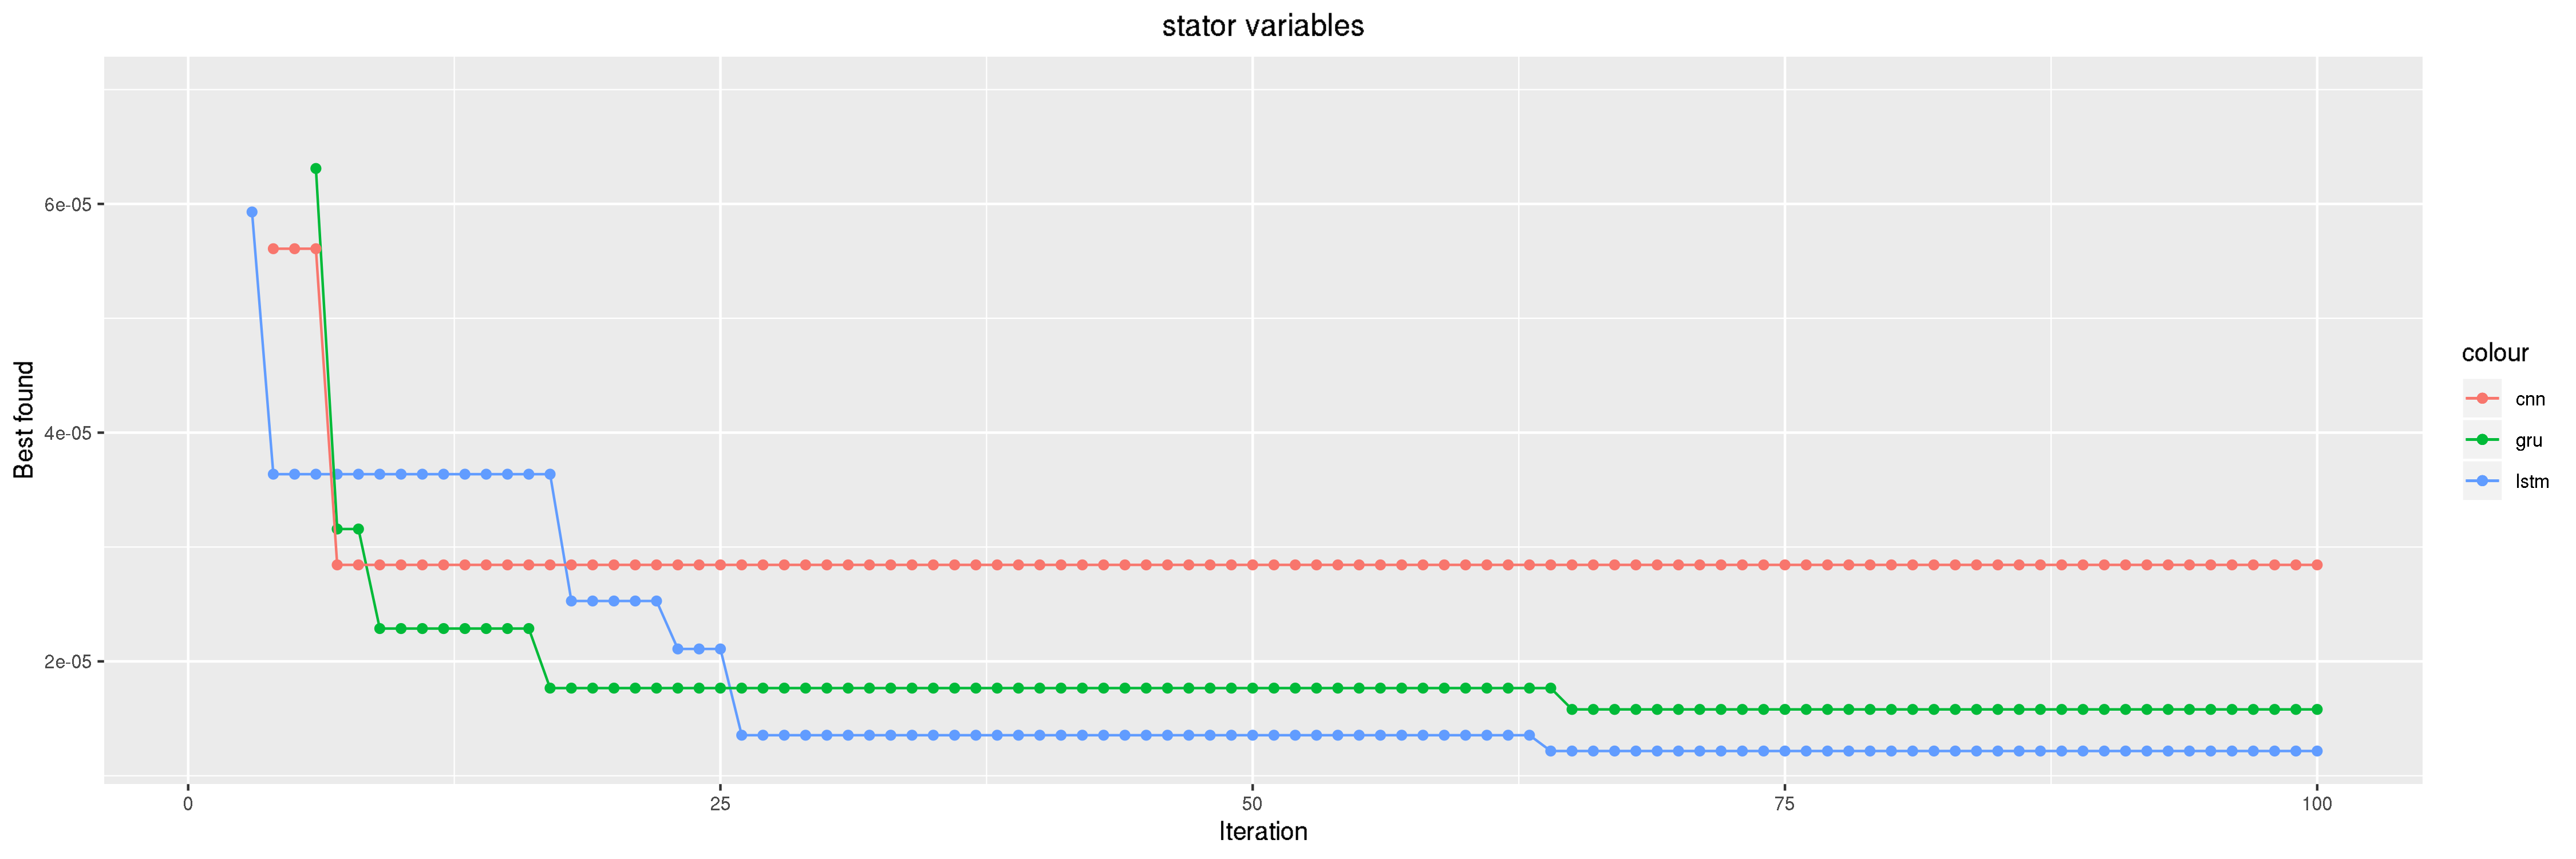
\includegraphics[width=\linewidth, height=4cm]{imgs/comparison_MSE_stator.png}
    \caption{Results of the optimization process on the pm and the three stator variables respectively using the MSE for the first task (RNN is excluded due to its poor performance). Values outside the specific range are excluded.}
    \label{fig:automl_mse}
\end{figure}
  
In addition, to improve predictions of critical temperatures, a custom weighted version of MSE is used as described in the previous section. Results of hyperparameter optimization with the new loss are shown in the Figure \ref{fig:automl_custom}.\\
\begin{figure}[!h]
    \centering
    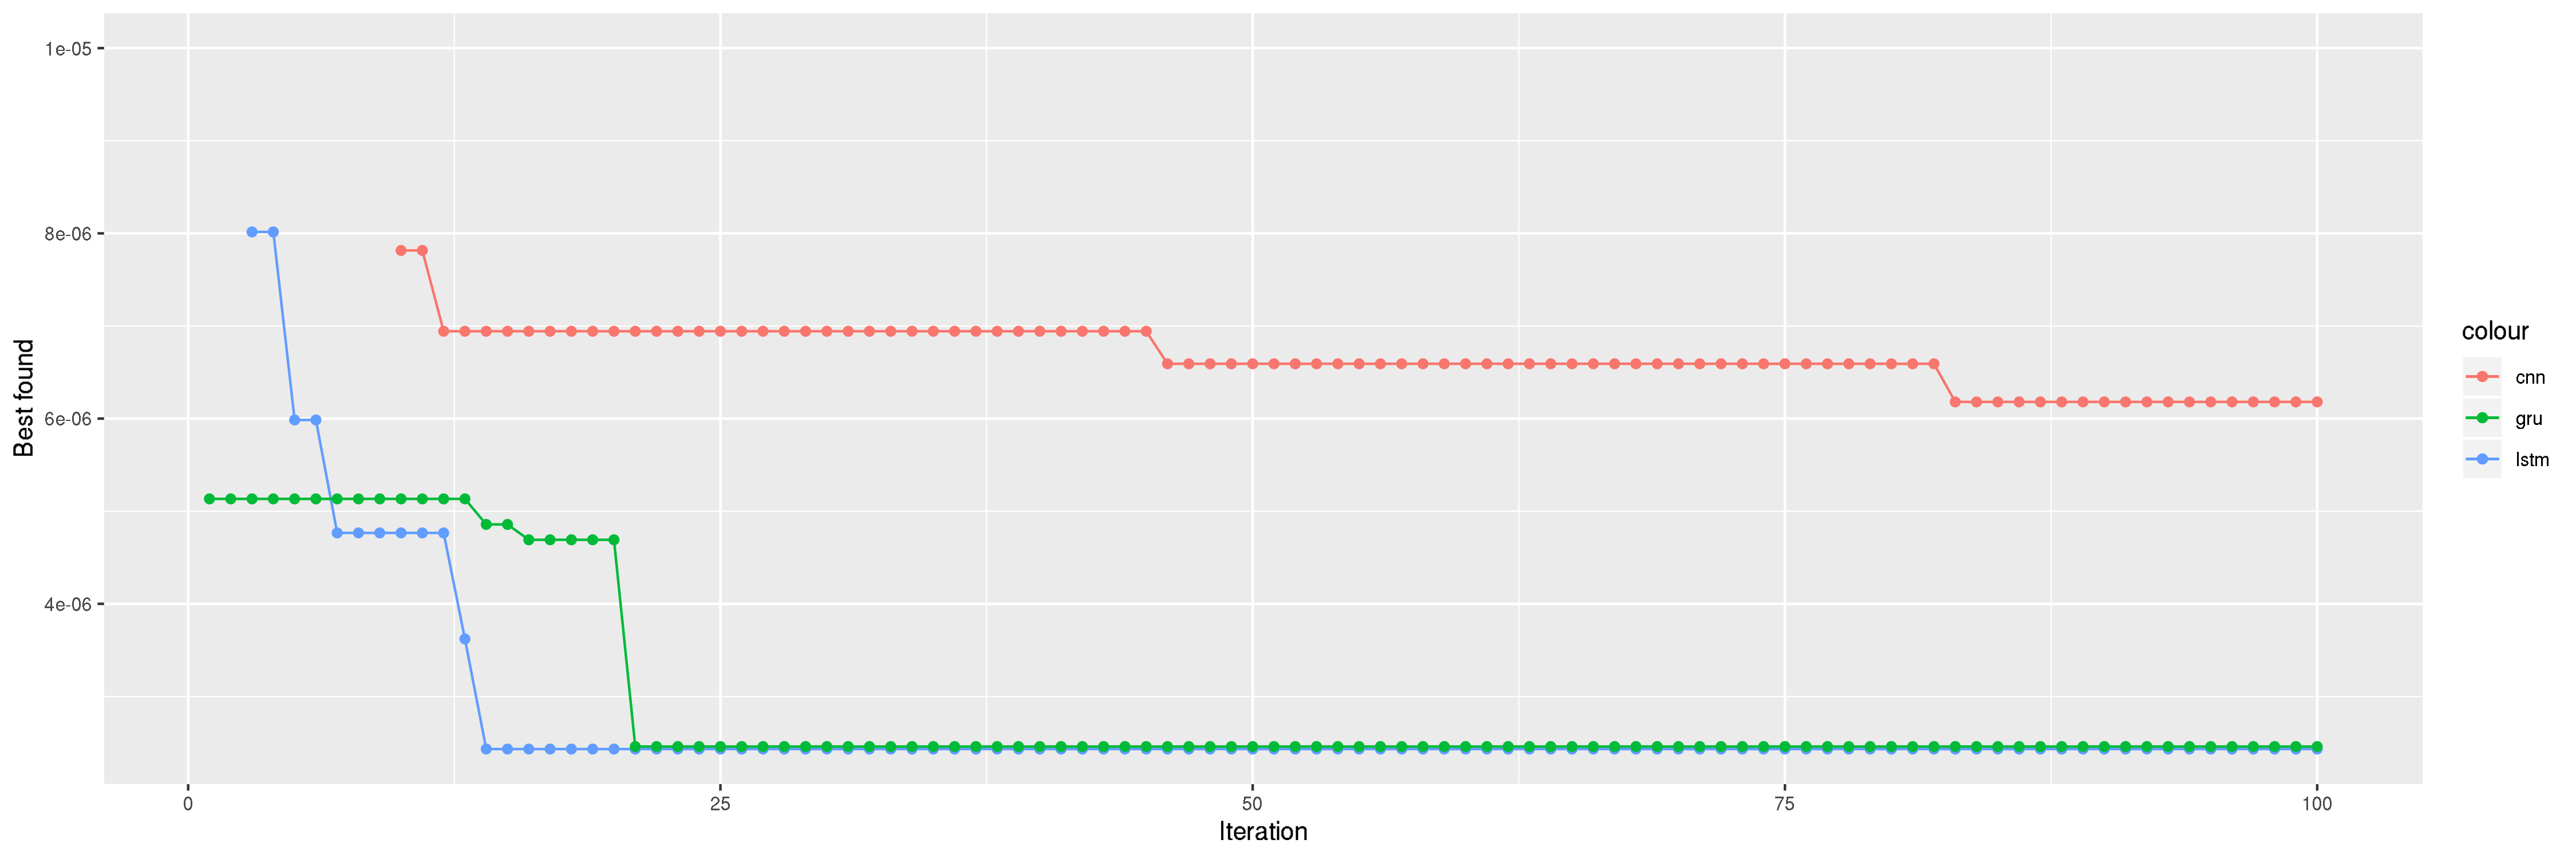
\includegraphics[width=\linewidth, height=4cm]{imgs/comparison_MSE_new_loss.png}
    \caption{Results of the optimization process using a custom loss for the first task (RNN is excluded due to its poor performance). Values outside the specific range are excluded.}
    \label{fig:automl_custom}
\end{figure}

%%NEED TO CREATE A  TABLE WITH THE TRAINING VALIDATION AND TEST RESULTS WITH BOTH LOSSES (ON THE SAME TABLE TO USE LESS SPACE).


\subsection{Second Task}
For the secondary task (predicting motor temperature without knowing previous values) results of hyperparameters optimization are shown in the figure \ref{fig:second_task}:
\begin{table}[!h]
  \centering
  \begin{tabular}{|l|c|c|c|c|c|c|}
    \hline
    & \multicolumn{3}{|c|}{MSE} & \multicolumn{3}{|c|}{Weighted MSE} \\
    \hline
    Models & Train & Validation & Test   & Train  & Validation & Test \\
    \hline
    RNN   & 0.0118 & 0.0127     & 0.0232 & 0.0131 & 0.0150     &  0.0254\\
    CNN   & 0.0121 & 0.0122     & 0.0126 & 0.0140 & 0.0142     & 0.0141\\
    LSTM  & 0.0143 & 0.0139     & 0.0149 & NA     & NA         & NA\\
    \hline
  \end{tabular}
  \caption{Results on Training, Validation and Test Set for the second task. Values can change (in a small range) due to stochasticity of algorithms.}
  \label{tab:first}
\end{table}

\begin{figure}[!h]
    \centering
    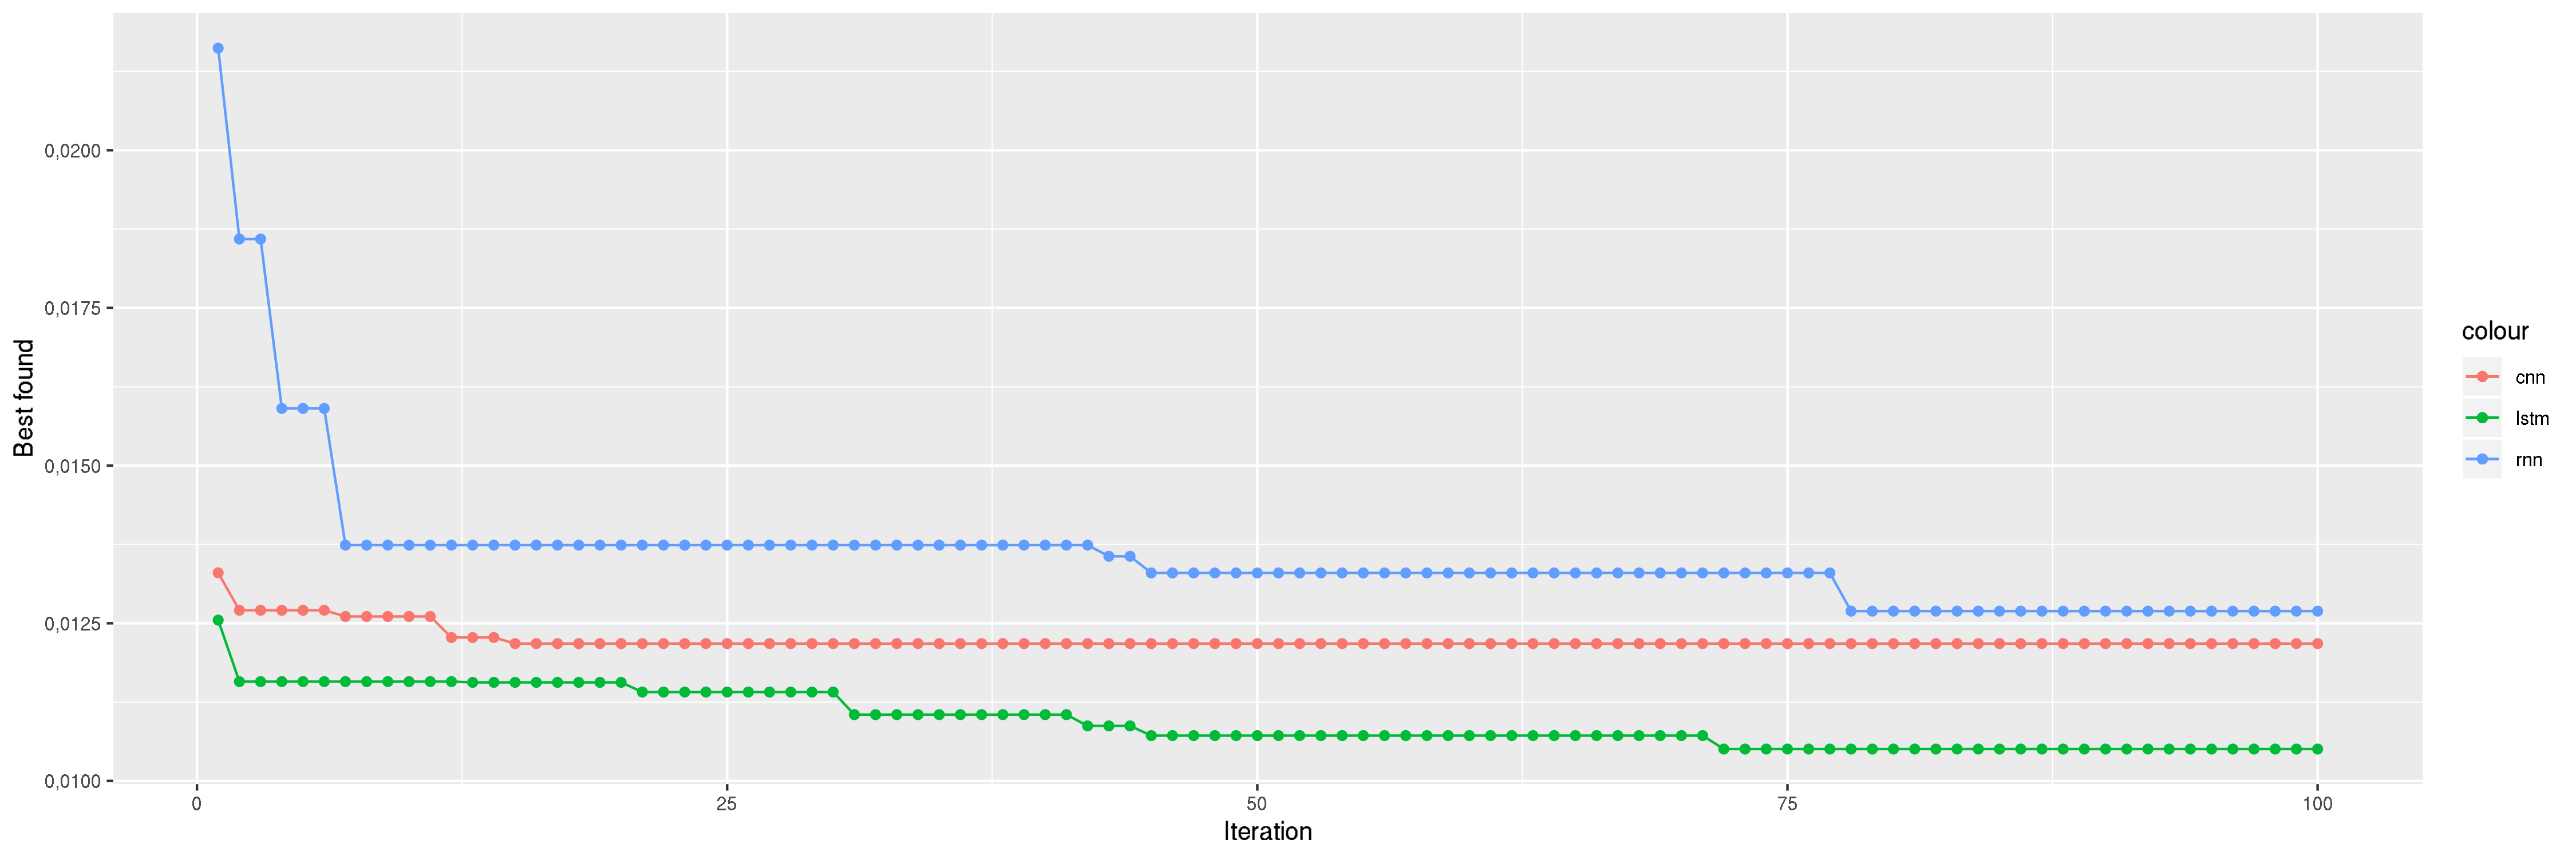
\includegraphics[width=\linewidth, height=4cm]{imgs/comparison_MSE_second.png}
    \caption{Result of the hyper-parameter optimization for the second task. Values outside the specific range are excluded.}
    \label{fig:second_task}
\end{figure}
  
% The Results section is dedicated to presenting the actual results (i.e. measured and calculated quantities), not to discussing their meaning or interpretation. The results should be summarized using appropriate Tables and Figures (graphs or schematics). Every Figure and Table should have a legend that describes concisely what is contained or shown. Figure legends go below the figure, table legends above the table. Throughout the report, but especially in this section, pay attention to reporting numbers with an appropriate number of significant figures. 

\section{Discussion}
As shown in Figure \ref{fig:automl_mse} and Figure \ref{fig:automl_custom}, after the optimization process, the LSTM and GRU yield the best results (LSTM is slightly better); CNN provides results comparable with these architecture, while RNN yields poor previsions when compared to the other architectures.

However, comparing results using only the loss value is not satisfying, because the model have to be light enough to be easily used by a car. So both number of parameters and performance are considered and plotted in the Figure
\begin{figure}[!h]
  \centering
  \begin{subfigure}[b]{0.4\linewidth} 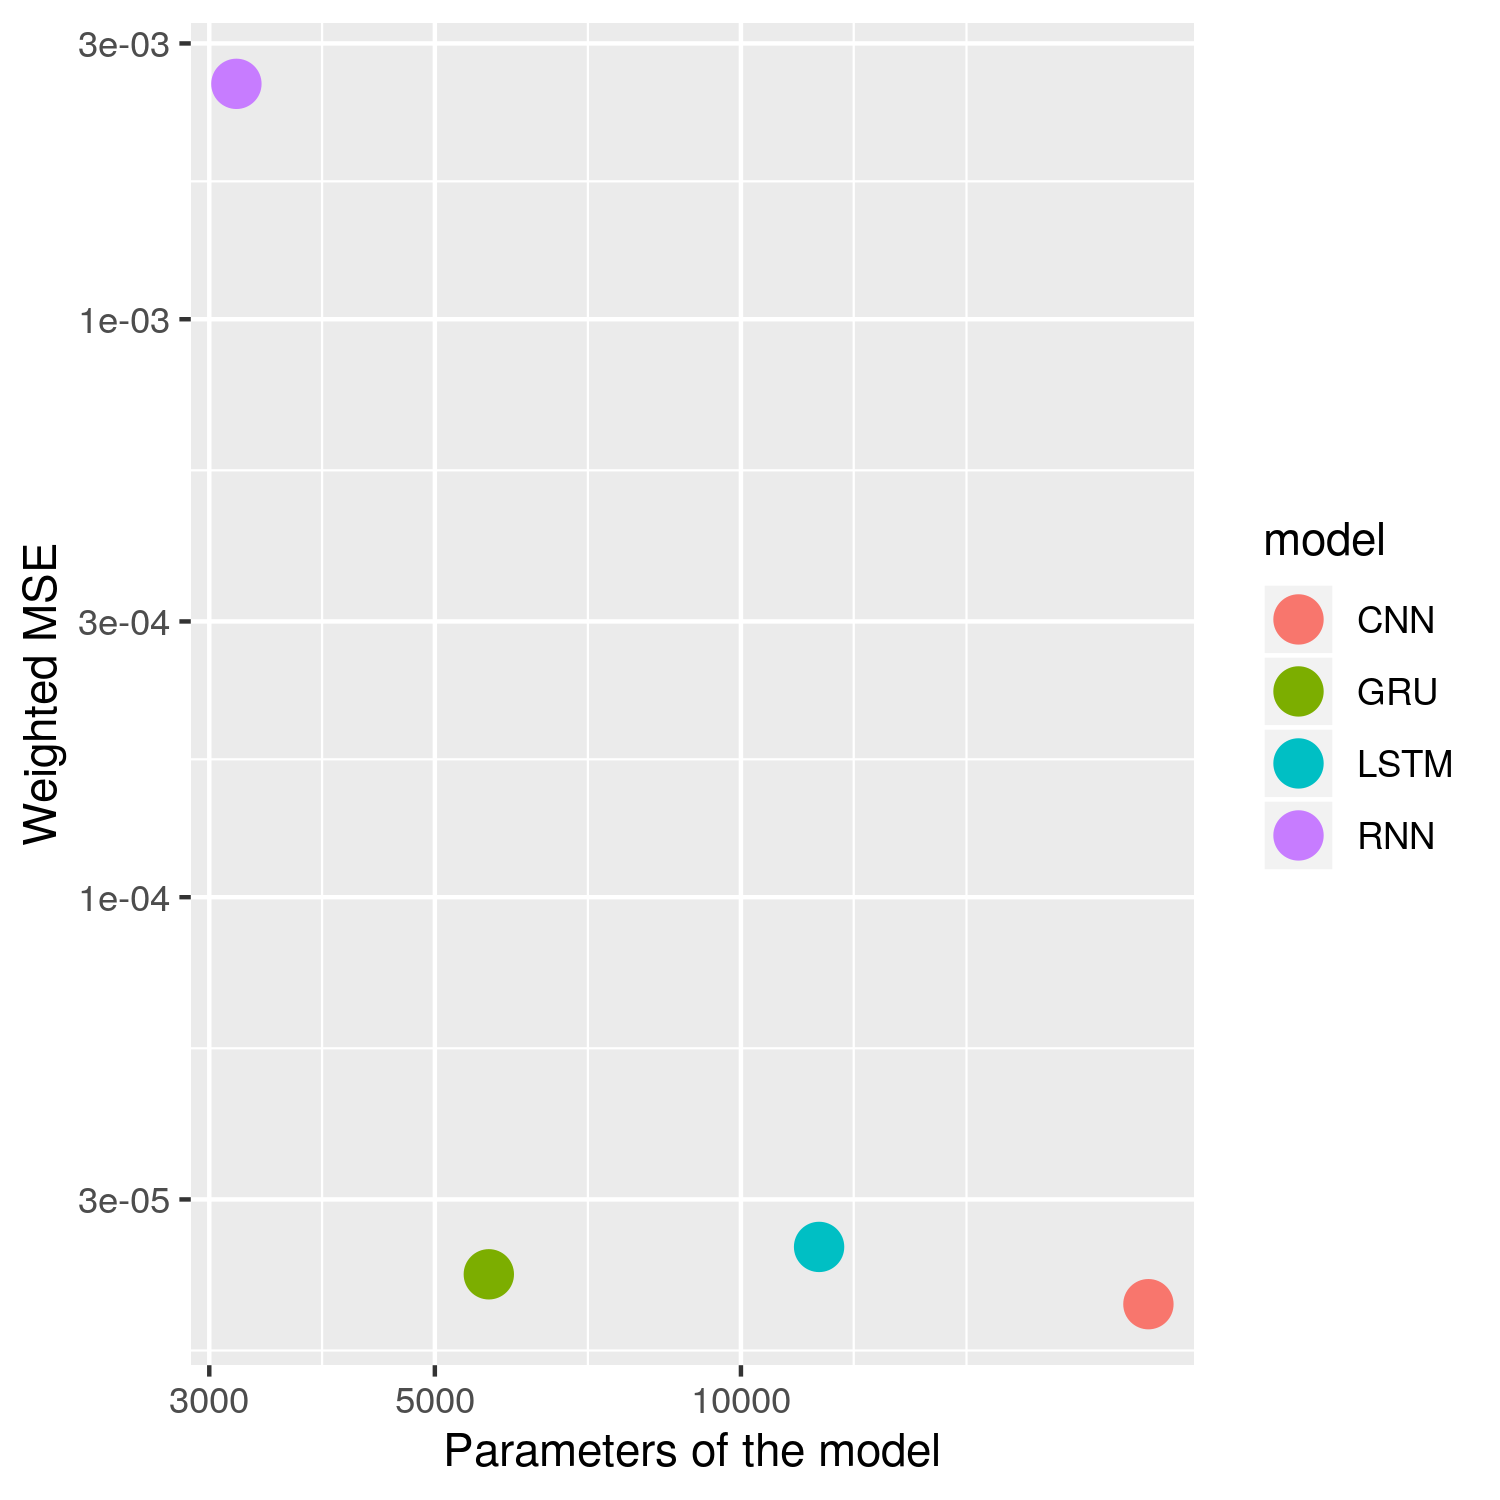
\includegraphics[width=\linewidth]{imgs/performance_parameters_Weighted_MSE1.png}
  \end{subfigure}
  \begin{subfigure}[b]{0.4\linewidth} 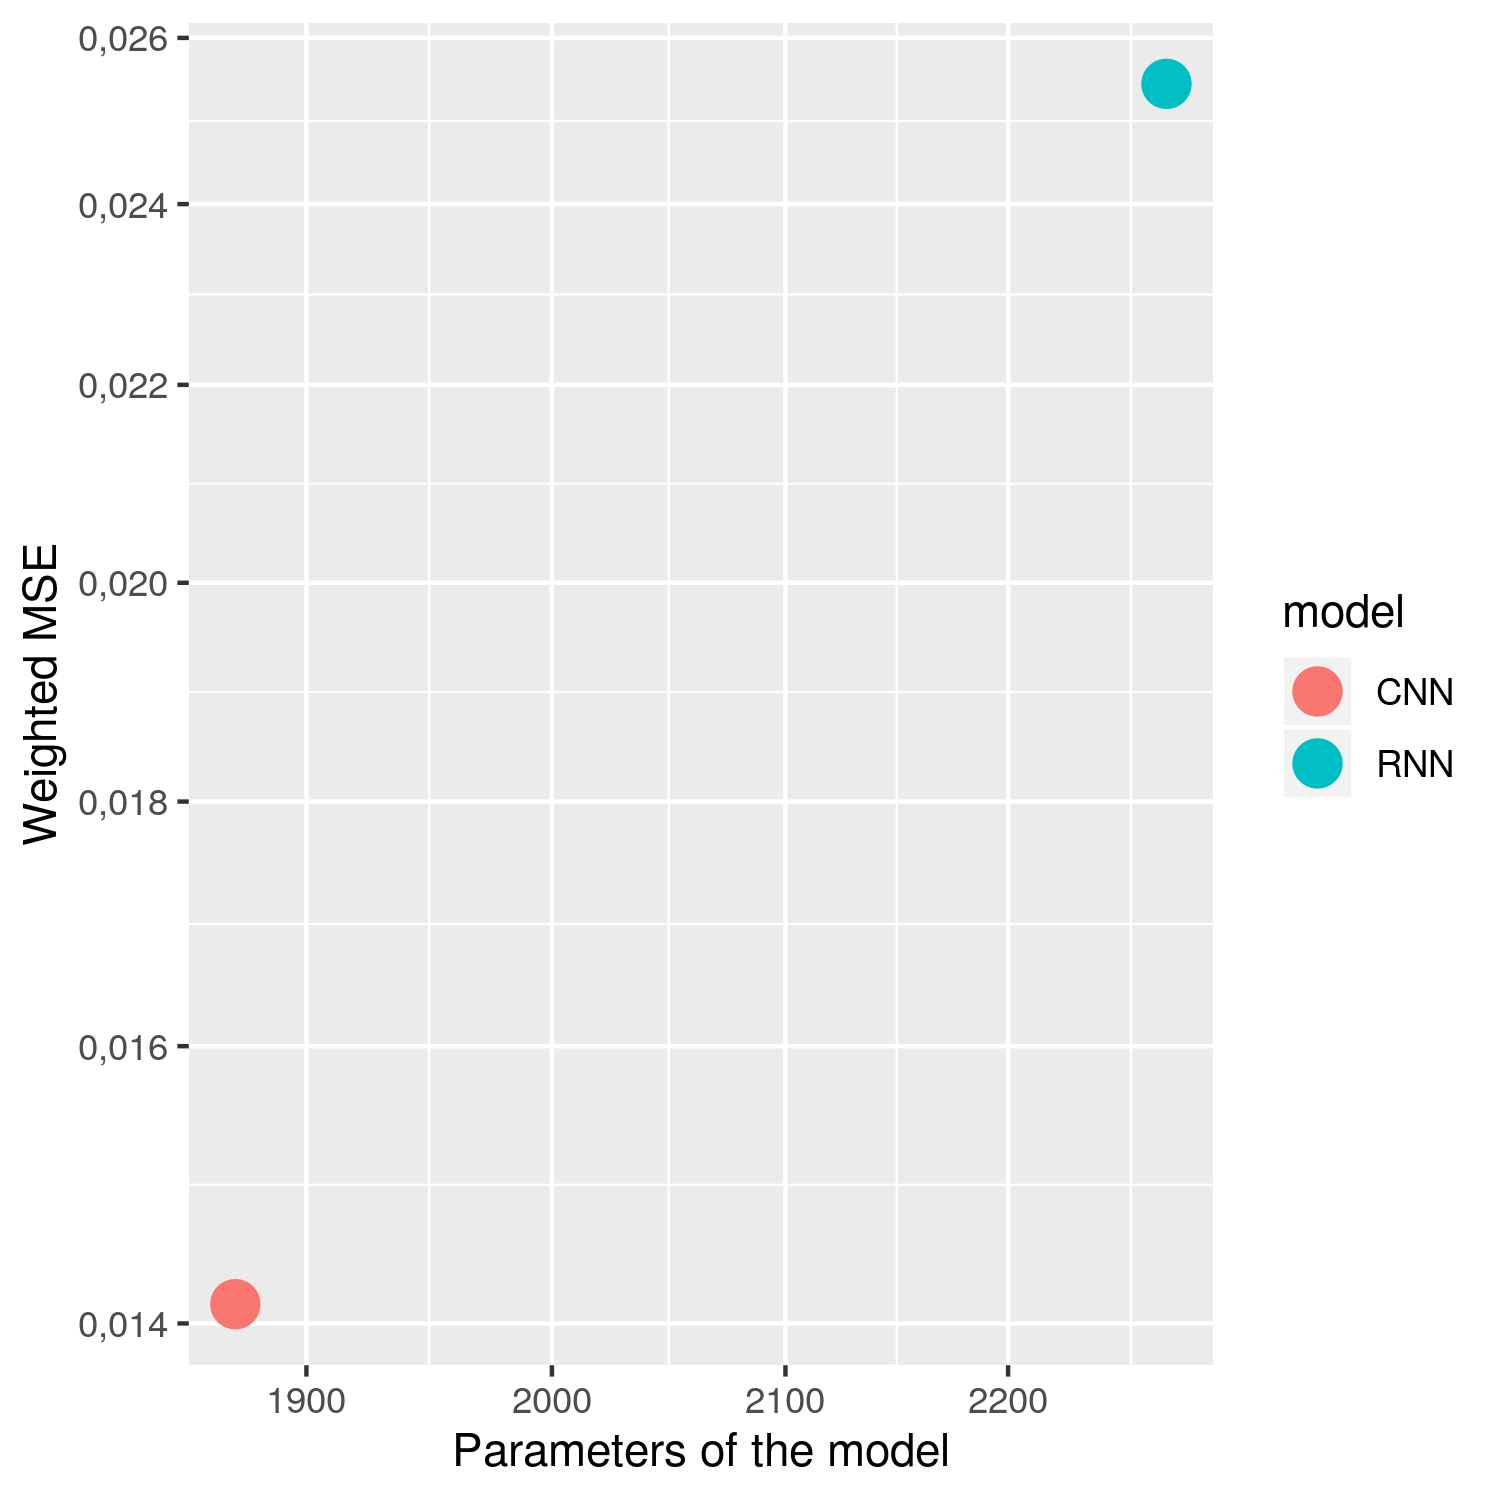
\includegraphics[width=\linewidth]{imgs/performance_parameters_Weighted_MSE2.png}
  \end{subfigure}
    \caption{Weighted MSE vs Number of parameters per model on the first (left) and second (rigth) task (on a logarithmic scale).}
    \label{fig:banana}
\end{figure}
  
As shown in Figure \ref{fig:banana}, numbers of parameters is one order of magnitude higher using the better architecture in the first task (CNN) instead of GRU, with little impact on prediction quality.
In the second task however, the most-accurate model has the minor number of parameters, so its use is not discutible. \newline

In the second task performances are pretty good for the \verb|stator| variables, but not so good for the \verb|pm| variable. The best model in this task is again the LSTM. The RNN's behavior is improved too.\\
In the prediction of the LSTM model on the test set (Figure \ref{fig:lstm_second}) a lot of noise can be noted in the prediction of the \verb|pm| variable.
The \verb|stator| variable prediction seems to follow the local trend pretty well, despite the fact that there is no direct formula connecting different physical quantities.

\begin{figure}[!h]
    \centering
    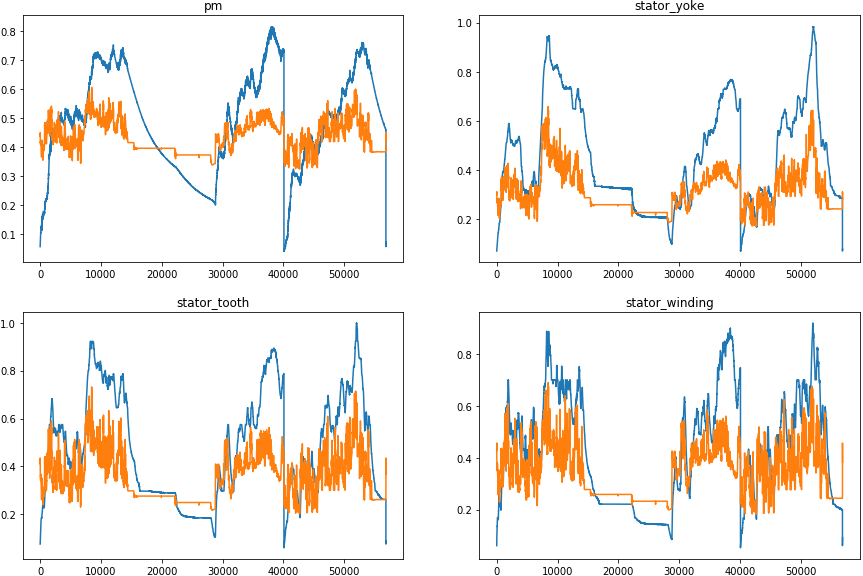
\includegraphics[width=\linewidth, height=4cm]{imgs/lstm_pred_second.png}
    \caption{Prediction of the LSTM model in the second task.}
    \label{fig:lstm_second}
\end{figure}


The weighted loss has been applied also in this case (with the CNN model) and it improves, as expected, the prediction for higher temperature as shown in Figure \ref{fig:cnn_second}. Prediction for lower and mid range temperature is more noisy, thus the overall MSE decreases.

\begin{figure}[!h]
    \centering
    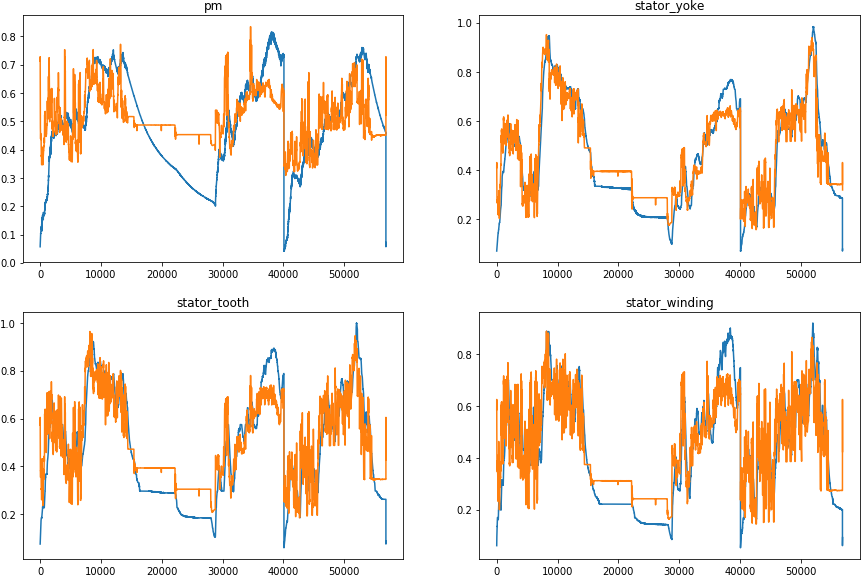
\includegraphics[width=\linewidth, height=4cm]{imgs/pred_second_custom_loss.png}
    \caption{Prediction of the CNN model in the second task with the custom loss.}
    \label{fig:cnn_second}
\end{figure}

Even creating a separate independent model for the \verb|pm| variable does not improve its performance.
Obtaining real data from actual cars might be useful to improve the model further: 
% All the data is produced in laboratory and addition of white noise, and
the AC current and voltage of the 3 phase reference system is supposed to be balanced, but all real systems have some irregularities, so a dq0 transformation is just a simplification of the problem.

% The discussion section aims at interpreting the results in light of the project's objectives. The most important goal of this section is to interpret the results so that the reader is informed of the insight or answers that the results provide. This section should also present an evaluation of the particular approach taken by the group. For example: Based on the results, how could the experimental procedure be improved? What additional, future work may be warranted? What recommendations can be drawn?


\section{Conclusions}
% BANANA STUFF,  IT'S AN ACTUAL BANANA!!
%                  \                                 (@@@@)
%                   \                               (@@@@@@)
%                    \                              (@@@@@@)
%                     \                              @@@@@@  
%                      \                             @@@@@   
%                       ------                      @@@@@@   
%                             \                    @@@@@@@@  
%                              \                  @@@@@@@@@@ 
%                               \               @@@@@@@@@@@@@
%                                --->          @@@@@@@@@@@@@@
%                                           @@@@@@@@@@@@@@@@@
%                                         @@@@@@@@@@@@@@@@@@@
%                                      @@@@@@@@@@@@@@@@@@@@@ 
%                                   @@@@@@@@@@@@@@@@@@@@@@@  
%                                @@@@@@@@@@@@@@@@@@@@@@@@@   
%                          @@@@@@@@@@@@@@@@@@@@@@@@@@@@@@    
%          @@@@@@@@@@@@@@@@@@@@@@@@@@@@@@@@@@@@@@@@@@@@      
% @@@@@@@@@@@@@@@@@@@@@@@@@@@@@@@@@@@@@@@@@@@@@@@@@@@        
% @@@@@@@@@@@@@@@@@@@@@@@@@@@@@@@@@@@@@@@@@@@@@@@@           
%   @@@@@@@@@@@@@@@@@@@@@@@@@@@@@@@@@@@@@@@@@@@              
%       @@@@@@@@@@@@@@@@@@@@@@@@@@@@@@@@@@@                  
%               @@@@@@@@@@@@@@@@@@@@                        
Recurrent models, since they are used for this kind of tasks, are expected to work well, but new trends in literature, such as \cite{cnn_time}\cite{cnn_time_2}, suppose that a CNN should also work well. This Project was a confirmation of this supposition: performance are at least comparable to recurrent models, if not better. \\
This report, however, cannot be a proof of them working better or worse because NAS was not done for either model, only the hyper parameter were optimized with a simple pseudo NAS where the number of layers can vary in some cases.

Target variables have a normal distribution when collected from different independent profiles, but in each profile the distribution is not normal, thus the optimal predictor for a series might not be linear, and the arima ACF/PACF plot has different ARIMA coefficients and components.
So, for each series a new ARIMA needs to be trained, making it unpractical to use; a deep learning model however generalizes well on all series, being a non-linear predictor.
If the model needs to be simplified even more, a great option would be an exponential smoothing model for the first task and a generalized linear regression for the second, given the high correlation among some of the variables, or even combining both models in a single one.

To improve the second task's performance, recurrent models can be used in a different way: after the prefixed lag number of event have taken place, the predicted values of past can be used with the model created in the first task to ``smoothen'' the model's prediction.

% Conclusions should summarize the central points made in the Discussion section, reinforcing for the reader the value and implications of the work. If the results were not definitive, specific future work that may be needed can be (briefly) described. The conclusions should never contain ``surprises''. Therefore, any conclusions should be based on observations and data already discussed. It is considered extremely bad form to introduce new data in the conclusions.

\section*{References}

% The references section should contain complete citations following standard form.  The references should be numbered and listed in the order they were cited in the body of the report. In the text of the report, a particular reference can be cited by using a numerical number in brackets as \cite{Lee2015} that corresponds to its number in the reference list. \LaTeX provides several styles to format the references

\bibliographystyle{IEEEtran}
% \nocite{*}
\bibliography{references}

\end{document}